% Tikz plot for UQ. This is based on the tikz code of
% Fabian Schuh for the tikz examples website
\documentclass[10pt,final,xcolor=dvipsnames,aspect ratio=169]{beamer}
%\usepackage{etex}

\usetheme{Madrid}

\usepackage{xspace}
%\usepackage{enumitem}
\usepackage[mathscr]{euscript}
\usepackage{subfigure}
\hypersetup{colorlinks,linkcolor=,urlcolor=blue}

% \usetheme{Boadilla}
% \usecolortheme{seahorse}

% the macros, packages, etc:
\usepackage[absolute,overlay]{textpos}
\setbeamertemplate{items}[ball]
\setbeamertemplate{blocks}[rounded][shadow=true]
\setbeamertemplate{navigation symbols}{}
\newenvironment{reference}[2]{%
  \begin{textblock*}{\textwidth}(#1,#2)
  \scriptsize{\it\color{black}}}{\end{textblock*}}
\setbeamertemplate{blocks}[rounded]% [shadow=false]
\newenvironment{boxalertenv}{\begin{altenv}%
      {\usebeamertemplate{alerted text begin}\usebeamercolor[fg]{alerted text}\usebeamerfont{alerted text}\colorbox{bg}}
      {\usebeamertemplate{alerted text end}}{\color{.}}{}}{\end{altenv}}

\usepackage{graphicx}
\usepackage{multirow,color}
\usepackage{bbm}
\usepackage{amsfonts,amsmath,amssymb,amsbsy,amsthm}
\usepackage{movie15}
\definecolor{themec}{RGB}{51,108,121}

%\usepackage{movie15}
%\usepackage{multimedia}
% custom commands (add your own macros here)

\definecolor{bronze}{rgb}{0.8, 0.5, 0.2}
\definecolor{goldenyellow}{rgb}{1.0, 0.87, 0.0}
\definecolor{amber}{rgb}{1.0, 0.75, 0.0}
\definecolor{azure}{rgb}{0.94, 1.0, 1.0}
\definecolor{bittersweet}{rgb}{1.0, 0.44, 0.37}
\definecolor{brass}{rgb}{0.71, 0.65, 0.26}
\definecolor{camel}{rgb}{0.76, 0.6, 0.42}
\setbeamercolor{block body}{bg=camel!30}
\usefonttheme[onlymath]{serif}
\usepackage{color}

\usepackage{amsmath}
\usepackage{mathtools}
\usepackage{tikz}
\usepackage{amsfonts,amsmath,amssymb,amsbsy,amsthm}
%\usecolortheme{tango}

%\usefonttheme{serif}     % Font theme: serif
%\usefonttheme[stillsansseriftext]{serif} 
%\renewcommand*\familydefault{\sfdefault}

\usepackage{pgf}
%\usepackage{pgfplots}
\usepackage{amssymb}
\usepackage{amsmath}
\usepackage{tikz}
\usepackage{verbatim}
%\usepackage{movie15}
\usepackage{tikz,pgfplots}
\setbeamertemplate{caption}{\raggedright\insertcaption\par}
%\usepackage[active,tightpage]{preview}
%\PreviewEnvironment{tikzpicture}
\usetikzlibrary{arrows,automata}
\usetikzlibrary{positioning}
\usetikzlibrary{fit}

%%%%%%%%%%%%%%%%%%%%%%%%%%%%%%%%%%%%%%%%%%%%%%%%%%%%%
%% this def file is based on the ccgodef
%%%%%%%%%%%%%%%%%%%%%%%%%%%%%%%%%%%%%%%%%%%%%%%%%%%%%
% packages
%\usepackage{booktabs}
%\usepackage[mathscr]{euscript}
%\usepackage{color}
%% mathdesgin or ams
%%\usepackage{amssymb,mathrsfs}
%\usepackage{graphicx}
%\usepackage{algorithmic,algorithm}
%\usepackage{tikz,pgfplots}
%\usepackage{upgreek}
%%\usepackage{showkeys,cite}
%\usepackage{multirow}
%\usepackage{yfonts}
%\usepackage{mathtools}
%\usepackage[normalem]{ulem}
%\usepackage{latexsym}
%\usepackage{url}
%\usepackage{amsmath,amssymb,amsbsy,amsfonts}
%\usepackage{enumitem}

\newcommand{\zapspace}{\topsep=0pt\partopsep=0pt\itemsep=0pt\parskip=0pt}

%% Notice macros
%\newcommand{\notice}[1]{\textcolor{Chameleon3}{#1}}
%\newcommand{\Notice}[1]{\textcolor{ScarletRed2}{#1}}
%\newcommand{\nnote}[1]{\noindent\emph{\textcolor{grass}{N: #1\,}}}
%\newcommand{\unote}[1]{\noindent\emph{\textcolor{blue}{U: #1\,}}}
%\newcommand{\onote}[1]{\noindent\emph{\textcolor{red}{O: #1\,}}}
%
%% colors
%\definecolor{utorange}{rgb}{0.8,0.33,0.}
%\definecolor{themec}{RGB}{51,108,121}
%\definecolor{darkred}{rgb}{.6,.1,.1}
%\definecolor{darkblue}{rgb}{.1,.1,.9}
%\definecolor{greenback}{rgb}{.19,.94,.13}
%\definecolor{orange}{rgb}{.76,.39,.13}
%\definecolor{grass}{rgb}{.19,.64,.13}
%\definecolor{sierp}{RGB}{209,28,209}
%\definecolor{bgorange}{rgb}{1.,.95,.78}
%\definecolor{grassgreen}{RGB}{92,135,39}
%\definecolor{thinbox}{rgb}{.7,.8,1.}

% general
\newcommand{\defeq}{\vcentcolon=}
%\newcommand{\del}[2]{\frac{\partial{#1}}{\partial{#2}}}
\renewcommand{\vec}[1]{{\mathchoice
                     {\mbox{\boldmath$\displaystyle{#1}$}}
                     {\mbox{\boldmath$\textstyle{#1}$}}
                     {\mbox{\boldmath$\scriptstyle{#1}$}}
                     {\mbox{\boldmath$\scriptscriptstyle{#1}$}}}}
\renewcommand{\ker}{\mathsf{ker}}
\newcommand{\ran}{\mathsf{range}}
\newcommand{\dom}{\mathsf{dom}}
\newcommand{\trace}{\mathsf{tr}}
\newcommand{\eps}{\varepsilon}
%\newcommand{\norm}[1]{\left\| {#1} \right\|}
\newcommand{\ip}[2]{{\left\langle {#1}, {#2} \right\rangle}}
\newcommand{\mip}[2]{\left\langle{#1}, {#2}\right\rangle_{\!\scriptscriptstyle{\text{M}}}}
\newcommand{\mat}[1]{\mathbf{{#1}}}
\newcommand\restr[2]{{
  \left.\kern-\nulldelimiterspace % automatically resize the bar with \right
  {#1}\vphantom{\big|} \right|_{#2}}}
\newcommand{\angles}[1]{\left\langle #1 \right\rangle}

% sets of numbers
\newcommand{\R}{\mathbb{R}}
\newcommand{\Z}{\mathbb{Z}}
\newcommand{\N}{\mathbb{N}}

\newcommand{\BB}{\mat{B}}
\newcommand{\Amat}{\mat{A}}
\newcommand{\VV}{\mat{V}}
\newcommand{\RR}{\mat{R}}

% commonly used mathcals
\newcommand{\A}{\mathcal{A}}
\newcommand{\B}{\mathcal{B}}
\newcommand{\C}{\mathcal{C}}
\newcommand{\D}{\mathcal{D}}
\newcommand{\E}{\mathcal{E}}
\newcommand{\F}{\mathcal{F}}
\newcommand{\G}{\mathcal{G}}
\newcommand{\J}{\mathcal{J}}
\newcommand{\U}{\mathcal{U}}
\newcommand{\Reg}{\mathcal{R}}

% shorthands
\newcommand{\bit}{\begin{itemize}}
\newcommand{\eit}{\end{itemize}}
\newcommand{\bdm} {\begin{displaymath}}
\newcommand{\edm} {\end{displaymath}}

% Probability (general)
\newcommand{\prob}{\mathsf{Prob}}
\newcommand{\borel}{\mathscr{B}}
\newcommand{\ave}{\mathsf{E}}
\newcommand{\GM}[2]{\mathcal{N}\!\left( {#1}, {#2}\right)}

% Bayesian stuff

\newcommand{\noisem}{\mu_{\text{noise}}}
\newcommand{\obs}{\vec{d}}
\newcommand{\ipar}{m}

\newcommand{\iparpr}{m_{\text{pr}}}
\newcommand{\iparref}{m_{\text{ref}}}
\newcommand{\iparmap}{m_{\scriptscriptstyle\text{MAP}}}
\newcommand{\dpar}{\vec{m}}
\newcommand{\dparmap}{\vec{m}_{\scriptscriptstyle\text{MAP}}}
%\newcommand{\priorm}{\mu_{\text{pr}}}
%\newcommand{\postm}{\mu_{\text{post}}}
\newcommand{\M}{\mat{M}}% the Mass matrix
%\newcommand{\ff}{\vec{f}}     % parameter-to-obs MAP
\newcommand{\ff}{\mathcal{F}} % parameter-to-obs MAP
\newcommand{\aff}{\tilde{\mathcal{F}}} % parameter-to-obs MAP
\newcommand{\noise}{\bs e}
\newcommand{\observables}{\bs d}
\newcommand{\data}{ \observables_{\rm{obs}} }
\newcommand{\uobs}{ \uu_{\rm{obs}} }
\newcommand{\datacomponent}[1]{ \observables_{\rm{obs}}^{#1} }
\newcommand{\FF}{{\ensuremath{\mat{F}}}}
\newcommand{\W}{{\ensuremath{\mat{W}}}}
\newcommand{\I}{{\ensuremath{\mat{I}}}}

\newcommand{\prior} {\pi_{\mbox{\tiny prior}}}
\newcommand{\like}{\pi_{\mbox{\tiny like}}}
\newcommand{\piobs}{\pi_{\mbox{\tiny obs}}}
\newcommand{\post}{\pi_{\mbox{\tiny post}}}
\newcommand{\pinoise}{\pi_{\mbox{\tiny noise}}}

\newcommand{\mupost}{\mu_{\mbox{\tiny post}}}
\newcommand{\muprior}{\mu_{\mbox{\tiny prior}}}

\newcommand{\ncov} {\bs{\Gamma}_{\!\mbox{\tiny noise}} }
\newcommand{\prcov} {\bs{\Gamma}_{\!\mbox{\tiny prior}} }
\newcommand{\postcov} {\bs{\Gamma}_{\!\mbox{\tiny post}} }
\newcommand{\aFF}{{\tilde{\ensuremath{\mat{F}}}}}
\newcommand{\ncovw} {\bs{W}}
\newcommand{\prcovr} {\bs{R}}

\newcommand{\Cprior}{\mathcal{C}_{\text{\tiny{prior}}}}
\newcommand{\Cpost}{\mathcal{C}_{\text{\tiny{post}}}}

\newcommand{\map} {{m}_{\mbox{\tiny MAP}} }
\newcommand{\dmap} {{\vec{m}}_{\mbox{\tiny MAP}} }
\newcommand{\mpr} {{\vec{m}}_{\mbox{\tiny pr}} }
\newcommand{\dbeta}{\vec{\beta}}
\newcommand{\dn}{\vec{n}}



\newcommand{\Hpost}  { \bs H }
\newcommand{\Hmisfit}{ \mat{H}_{\mbox{\tiny misfit}} }
\newcommand{\tHmisfit}{\tilde{\mat{H}}_{\mbox{\tiny misfit}} }
\newcommand{\HT}{\matrix{\tilde{H}}_{\mbox{\tiny misfit}}}
\newcommand{\HTinf}{\tilde{H}_{\text{misfit}}}
\newcommand{\Vr} {\bs V_r}
\newcommand{\Dr} {\bs D_r}
\newcommand{\Ir} {\bs I_r}

%\newcommand{\Ge}{ \ensuremath{\matrix{G}}_{\!\mbox{\tiny e}}}
%\newcommand{\Op}{ \ensuremath{\matrix{O}}_{\!\mbox{\tiny p}}}
\newcommand{\Ge}{ \mathcal{G}_{\!\mbox{\tiny e}}}
\newcommand{\Op}{ \mathcal{O}_{\!\mbox{\tiny p}}}
\newcommand{\HH}{ \ensuremath{\matrix{H}} }
\newcommand{\SI}{ \ensuremath{{\Sigma}} }
\newcommand{\PP}{ \ensuremath{\matrix{\Psi}} }
%\newcommand{\WW}{ \ensuremath{\matrix{W}} }
\newcommand{\WW}{ \mathcal{W}}

% Macros for three different forms of adjoint operator
\newcommand{\adjMacroMM}[1]{{#1}^*}
\newcommand{\adjMacroME}[1]{{#1}^\natural}
\newcommand{\adjMacroEM}[1]{{#1}^\diamond}
\newcommand{\adjMacroEMINV}[1]{{#1}^{-\diamond}}
\newcommand{\Aadj}{\adjMacroMM{\A}}
\newcommand{\Badj}{\adjMacroMM{\BB}}
\newcommand{\iFadj}{\adjMacroME{\iF}}
\newcommand{\Fadj}{\adjMacroME{\F}}
\newcommand{\Vadj}{\adjMacroEM{\VV}}
\newcommand{\Ladj}{\adjMacroEM{\L}}

\def\bfG{\mbox{\boldmath$G$}}
\newcommand{\mc}[1]{\mathcal{#1}}

%%%%%%%%%%%%%%%%%%%%%%%%%%%%%%%%%%%%
% custom commands to the sc14 paper
%%%%%%%%%%%%%%%%%%%%%%%%%%%%%%%%%%%%
\newcommand{\SNR}{\ensuremath{\text{SNR}}}

\newcommand{\gbf}[1]{\boldsymbol{#1}}
\newcommand{\bs}[1]{\ensuremath{\boldsymbol{#1}}}

\newcommand{\edot}{\dot{\gbf{\varepsilon}}}
\newcommand{\edotsec}{\edot_\mathrm{II}}
\newcommand{\secinve}{\edot_\mathrm{II}}

\DeclareMathOperator{\sym}{sym}
%\DeclareMathOperator{\trace}{tr}
%\DeclareMathOperator{\diag}{diag}

\newcommand{\Div}{\mbox{div}}
\newcommand{\Grad}{{\bf \nabla}}
\newcommand{\grad}{\nabla}

\newcommand{\pt}{\tilde{p}}
\newcommand{\vt}{\tilde{\vv}}
\newcommand{\qt}{\tilde{q}}
\newcommand{\betat}{\tilde{\beta}}

\newcommand{\uh}{\hat{\uu}}
\newcommand{\ph}{\hat{p}}
\newcommand{\vh}{\hat{\vv}}
\newcommand{\qh}{\hat{q}}
\newcommand{\betah}{\hat{\beta}}

\renewcommand{\vec}[1]{\gbf{#1}}
\newcommand{\cvec}[1]{{#1}}

\newcommand{\uu}{\ensuremath{\vec{u}}}
\newcommand{\vv}{\ensuremath{\vec{v}}}

\definecolor{darkblue}{rgb}{.1,.1,.9}
\definecolor{utorange}{rgb}{0.8,0.33,0.}
% this are only needed for presentations
\newcommand{\tcb}[1]{\textcolor{blue}{{#1}}}
\newcommand{\tcdb}[1]{\textcolor{utorange}{{#1}}}
\newcommand{\tcr}[1]{\ensuremath{\textcolor{red}{{#1}}}}
\newcommand{\tcdr}[1]{\textcolor{darkred}{{#1}}}
\newcommand{\tcm}[1]{\textcolor{ForestGreen}{{#1}}}
\newcommand{\tcmag}[1]{\textcolor{magenta}{{#1}}}
\newcommand{\tco}[1]{\textcolor{VioletRed}{{#1}}}
\newcommand{\tcc}[1]{\textcolor{cyan}{{#1}}}
\newcommand{\dg}[1]{\textcolor{black!65!green}{{#1}}}
\newcommand{\tcg}[1]{\textcolor{blue!70!black!30!green}{{#1}}}
\newcommand{\tcdg}[1]{\textcolor{blue!20!black!50!green}{{#1}}}
\newcommand{\tcch}[1]{\textcolor{cyan}{\hat{{#1}}}}
\newcommand{\tcmhb}[1]{\textcolor{magenta}{\hat{\gbf{{#1}}}}}
\newcommand{\tcmh}[1]{\textcolor{magenta}{\hat{{#1}}}}
\newcommand{\tcbb}[1]{\textcolor{blue}{\gbf{{#1}}}}
\newcommand{\tcgb}[1]{\textcolor{grass}{\gbf{{#1}}}}
\newcommand{\tcct}[1]{\textcolor{cyan}{\tilde{{#1}}}}
\newcommand{\tcmtb}[1]{\textcolor{magenta}{\tilde{\gbf{{#1}}}}}
\newcommand{\tcmt}[1]{\textcolor{magenta}{\tilde{{#1}}}}
\newcommand{\tcotb}[1]{\textcolor{utorange}{\tilde{\gbf{{#1}}}}}
\newcommand{\tcot}[1]{\textcolor{utorange}{\tilde{{#1}}}}
\newcommand{\tcohb}[1]{\textcolor{utorange}{\hat{\gbf{{#1}}}}}
\newcommand{\tcoh}[1]{\textcolor{utorange}{\hat{{#1}}}}

\renewcommand{\matrix}[1] {\ensuremath{\boldsymbol{#1}}}

\newcommand{\bndFS}{\Gamma_{\!\mbox{\scriptsize $FS$}}}
\newcommand{\bndB}{\Gamma_{\!\mbox{\scriptsize $B$}}}
\newcommand{\bndT}{\Gamma_{\!\mbox{\scriptsize $T$}}}

\usepackage{xspace}
\newcommand{\software}[1]{\texttt{#1}\xspace}
\newcommand{\hip}{\texttt{hIPPYlib}\xspace}
\newcommand{\bhip}{\texttt{{\bf hIPPYlib}}\xspace}
\newcommand{\Fe}{\texttt{FEniCS}\xspace}
\newcommand{\pet}{\texttt{PETSc}\xspace}


\newcommand{\del}{\partial}
%\newcommand{\D}{\mathcal{D}}
\newcommand{\Ns}{{N_s}}
\newcommand{\Ntau}{{N_{\tau}}}
\newcommand{\iFF}{\mathcal{F}}
%\newcommand{\priorm}{\muprior}
\newcommand{\Acal}{\mc{A}}
%\newcommand{\postm}{\mupost}
\newcommand{\iparpost}{\ipar_\text{post}}
\newcommand{\dd}{\vec{\bar{d}}}
\newcommand{\obsop}{\mathcal{B}}

\newcommand{\GN}{\ensuremath{\Gamma_{\!\!N}}}
\newcommand{\Exp}[1]{e^{{#1}}}
\newcommand{\GD}{\ensuremath{\Gamma_{\!\!D}}}
\newcommand{\Vg}{\mathscr{V}_{\!g}}
\newcommand{\V}{\mathscr{V}_{\!\scriptscriptstyle{0}}}
\newcommand{\eip}[2]{\left\langle{#1}, {#2}\right\rangle_{\!{\R^q}}}
\newcommand{\Wn}{\mat{W}_{\!\sigma}}
\newcommand{\cip}[2]{\left\langle{#1}, {#2}\right\rangle_{\!\CM}}
\newcommand{\CM}{\mathscr{E}}
\newcommand{\LI}{\mathscr{L}}
\renewcommand{\H}{\mathcal{H}}
\newcommand{\Nd}{{n_{\text{d}}}}
\newcommand{\Ntr}{{n_{\text{tr}}}}
\newcommand{\ipart}{m_{\scriptscriptstyle\text{true}}}
\newcommand{\ut}[1]{\ensuremath{\tilde{#1}}}

\newcommand{\LRp}[1]{\left( #1 \right)}
\newcommand{\LRs}[1]{\left[ #1 \right]}
\newcommand{\LRa}[1]{\left< #1 \right>}
\newcommand{\LRc}[1]{\left\{ #1 \right\}}

\newcommand{\xx}{\ensuremath{\boldsymbol x}}
\newcommand{\rr}{\ensuremath{\boldsymbol r}}
\newcommand{\e}{\ensuremath{\boldsymbol e}}
\newcommand{\x}{\xx}
\newcommand{\y}{\ensuremath{\boldsymbol y}}
\newcommand{\z}{\ensuremath{\boldsymbol z}}
\renewcommand{\r}{\ensuremath{\boldsymbol r}}
\newcommand{\s}{\ensuremath{\boldsymbol s}}

\newcommand{\hilb}{\mathscr{H}}
\newcommand{\half} {\ensuremath{\frac{1}{2}}}
\newcommand{\nor}[1]{\left\| #1 \right\|}
\newcommand{\equaldef}{{:=}}
\newcommand{\iFFadj}{\adjMacroMM{\iFF}}

\newcommand{\istate}{u}
\newcommand{\iparspace}{\mathcal{M}}
\newcommand{\iadj}{p}
\DeclareMathOperator*{\argmin}{argmin} 
\DeclareMathOperator{\diag}{diag} 


\newcommand{\err}{\vec{\eta}}
\newcommand{\beps}{\bs{\eps}}
\newcommand{\bbeps}{\bar{\bs{\eps}}}
\newcommand{\bnu}{\bs{\nu}}
\newcommand{\ncovbeps} {\bs{\Gamma}_{\!\mbox{\tiny \beps}} }
\newcommand{\ncovbnu} {\bs{\Gamma}_{\!\mbox{\tiny \bnu}} }
\newcommand{\norm}[2][]{\left\Vert #2\right\Vert_{#1}}
\newcommand{\dbetamap}{\vec{\beta}_{\scriptscriptstyle\text{MAP}}}
\newcommand{\betamap}{{\beta}_{\scriptscriptstyle\text{MAP}}}
\newcommand{\smallB}{\scriptscriptstyle\text{B}}
\definecolor{lightblue}{cmyk}{0.88,0.44,0,0.07}
\newcommand{\betapr}{\beta_{\text{pr}}}
\newcommand{\ntrue}{a_{\scriptscriptstyle\text{true}}}
\newcommand{\NoiseForcing}{\xi}
\newcommand{\ProbMeasClass}{\mathcal{P}}
\newcommand{\ProbMeas}{\mathbbm{P}}
\newcommand{\SigmaAlg}{F}

\newcommand{\Hmatrix}{\bs{H}}

\newcommand{\iparb}{\bar{\ipar}}
\newcommand{\euclidnorm}[1]{\left\| {#1} \right\|_2}
\newcommand{\incu}{\upupsilon}
\newcommand{\incp}{\uprho}
\newcommand{\QoIquad}{\QoI_\text{quad}}
\newcommand{\tcblue}[1]{\textcolor{blue}{#1}}
\newcommand{\betad}{\bs{\beta}}

\newcommand{\preconditioner}{\widetilde{H}}
\newcommand{\impulseresponse}{\phi}
\newcommand{\spatialmean}{\mu}
\newcommand{\Aop}{\mathcal{A}}
\newcommand{\btVFill}{\vskip0pt plus 1filll}
\tikzset{
    state/.style={
           rectangle,
           rounded corners,
           draw=black, very thick,
           minimum height=3em,
           inner sep=1pt,
           text centered,
           },
}

\newcommand{\Aker}{\Phi}
%\DeclareMathOperator{\diag}{diag}
%\newcommand{\Hmatrix}{\bs{H}}
\newcommand{\Hm}{\mathcal{H}}

% argument #1: any options
\newenvironment{customlegend}[1][]{%
    \begingroup
    % inits/clears the lists (which might be populated from previous
    % axes):
    \csname pgfplots@init@cleared@structures\endcsname
    \pgfplotsset{#1}%
}{%
    % draws the legend:
    \csname pgfplots@createlegend\endcsname
    \endgroup
}
\def\addlegendimage{\csname pgfplots@addlegendimage\endcsname}

% title, authors, etc:
\title[Local PSF high-rank Hessian approximation]{Local Point Spread Function Approximation of High-Rank Hessians in Inverse Problems Governed by	PDEs\thanks{Research supported
    partially by NSF-DMS-CAREER-1654311 and NSF-OAC-1550547.}}
%\author[{Noemi
%    Petra}]{No\'{e}mi~Petra\inst{1}}

\author[Tucker Hartland]{{Tucker Hartland}\inst{1}\\[2ex]
  {\small \textcolor{themec}{Joint work with:}}
  \\
  {\small Nick Alger}\inst{2},
  {\small No{\'e}mi Petra}\inst{3},
  {\small Omar Ghattas}\inst{2}
}

\institute[LLNL]{%
  \inst{1}{Center for Applied Scientific Computing, Lawrence Livermore National Laboratory}\\\smallskip
  \inst{2}{Oden Institute for Computational Engineering and Sciences, The University of Texas at Austin}\\\smallskip
  \inst{3}{Department of Applied Mathematics, University of California, Merced}
}

\date[March 5, 2024]
     {\footnotesize 
     	MS11
     	HPC Algorithms for Inverse Problems and Digital Twins \\
     	SIAM Conference on Parallel Processing for Scientific Computing (PP24) \\
       Tuesday, March 5}

 \begin{document}

 % -------------------------------------------------------------------
%%\AtBeginSubsection[]  % "Beamer, do the following at the start of every section"
%\AtBeginSection[]  % "Beamer, do the following at the start of every section"
%{
%  \begin{frame}<beamer>
%    \frametitle{Outline} % make a frame titled "Outline"
%    \small
%  %\tableofcontents[currentsubsection]  % show TOC and highlight current section
%  \tableofcontents[currentsection]  % show TOC and highlight current section
%\end{frame}
%}
%----------- titlepage ----------------------------------------------%
\begin{frame}[plain]
  \titlepage
\end{frame}


%-------------------------------------------------------------------
\begin{frame}
	\frametitle{Need predictive models with quantified uncertainties to accurately anticipate future sea
		level rise.}
	%\framesubtitle{Sea level projections from the IPCC 6th Assessment Report, 2021}
	%\vspace{0.2in}
	\begin{columns}
		\begin{column}{0.7\paperwidth}
			\centering\includegraphics[width=0.75\columnwidth]{extraplots/venezia}
		\end{column}
		\hspace{-0.4in}
		\begin{column}{0.3\paperwidth}
			\vspace{0.1in}
			\centering\includegraphics[width=0.75\columnwidth]{extraplots/ipcc-ar6-wgi-2021.png}
		\end{column}
	\end{columns}
	
	%\centering\includegraphics[width=0.55\columnwidth]{extraplots/nasa-sea-level-projection-tool.png}
	
	\vspace{0.1in}
	%\begin{block}{IPCC Fourth Assessment Report: Climate Change 2007}
	%  {\small
	%    {\em [T]he uncertainty in the projections of the land ice
	%      contributions [to sea level rise] is dominated by the various
	%      uncertainties in the land ice models themselves
	%      ... rather than in the temperature projections.''} %[10.A.6]
	%  }
	%\end{block}
	\begin{itemize}
		\item Several port cities will be at risk from coastal
		flooding in the future.
		\item Ice flowing from ice sheets to ocean is primary contributor
		to sea level rise.
	\end{itemize}
	
	\begin{itemize}
		\item [] \scriptsize{Details in: Masson-Delmotte, V. et al. ``IPCC,
			2021: Summary for Policymakers. In: Climate Change 2021: The
			Physical Science Basis. Contribution of Working Group I to the
			Sixth Assessment Report of the Intergovernmental Panel on Climate
			Change'', Cambridge University Press. In Press.}
	\end{itemize}
	
	
	
\end{frame}


\begin{frame}
	\frametitle{Motivation: inversion for continental scale ice sheet models}
	
	\vspace{0.2in}
	\begin{columns}
		\begin{column}{0.47\paperwidth}
			\centering\includegraphics[width=0.7\columnwidth]{extraplots/ScienceRignot-crop.pdf}
			%\vspace{-0.2in}
			\vspace{-0.1in}
			\begin{center}
				{\scriptsize Observed surface flow velocity from InSAR \\
					\vspace{-0.05in}
					(Rignot et.\ al, 2011)}
			\end{center}
		\end{column}
		\hspace{-0.4in}
		\begin{column}{0.51\paperwidth}
			\vspace{0.15in}
			
			\centering\includegraphics[width=0.8\columnwidth]{extraplots/beta_cube_cut.png}
			
			\vspace{0.1in}
			\begin{center}
				{\scriptsize Antarctic ice sheet inversion \\ for the basal friction parameter field \\
					\vspace{-0.05in}
					from InSAR surface velocities}
			\end{center}
		\end{column}
	\end{columns}
	
	%\vspace{0.3in}
	\btVFill
	
	\scriptsize{Details in: T. Isaac, N. Petra, G. Stadler, and
		O. Ghattas. {\em Scalable and efficient algorithms for the
			propagation of uncertainty from data through inference to
			prediction for large-scale problems, with application to flow of
			the Antarctic ice sheet}, Journal of Computational Physics, 296,
		348-368 (2015).}
	%	\begin{block}{IPCC Fourth Assessment Report: Climate Change 2007}
	%		{\small
	%			{\em [T]he uncertainty in the projections of the land ice
	%				contributions [to sea level rise] is dominated by the various
	%				uncertainties in the land ice models themselves
	%				... rather than in the temperature projections.} %[10.A.6]
	%		}
	%	\end{block}
\end{frame}


\begin{frame}[t]
	\frametitle{Outline}
	
	\begin{itemize}
		\setlength\itemsep{1.0em}
		\item Motivation
		\vspace{0.02in}
		\begin{itemize}
			\setlength\itemsep{1.0em}
			\item Predictive continental scale ice sheet models for anticipating future sea level rise with quantified uncertainties
			\vspace{0.02in}
			\item The need to go beyond ``low rank'' Hessian approximations
		\end{itemize}
		%\vspace{0.02in}
		%\item Bayesian inverse problems governed by PDEs (preliminaries)
		\vspace{0.02in}
		\item Exploiting structured low-rank properties of (Bayesian) inverse problems governed by PDEs
		\vspace{0.02in}
		\begin{itemize}
			\setlength\itemsep{1.0em}
			\item (Global) low rank approximation
			\vspace{0.02in}
			\item Hierarchical off-diagonal low rank (HODLR) approximation
			\vspace{0.02in}
			\item A local point spread function method as a means for efficient
			$\mathcal{H}$ierarchical-matrix approximation
		\end{itemize}
		\vspace{0.02in}
		\item Example: Inversion for the basal friction
		coefficient field in an ice sheet flow problem
		\vspace{0.02in}
		\item Conclusions
	\end{itemize}
	
\end{frame}



\begin{frame}
	\frametitle{Ice sheet dynamics}
	\framesubtitle{Stokes model}	
	\begin{block}{Balance of mass and linear momentum}
		\[
		\begin{aligned}
		% balance of linear momentum:
		- \gbf{\nabla} \cdot \gbf{\sigma}
		%\left[
		% \eta(\gbf{u}) \, \edot
		%-\gbf{I}p \right]
		&= \rho\, \gbf{g},
		&&[
		\gbf{\sigma}=\eta(\gbf{u}) \, \edot - \gbf{I}p]
		%\edot = \tfrac 12  (\gbf{\nabla u} + \gbf{\nabla  u}^{\top})]
		\hspace{-2em}
		\\
		% balance of mass:
		\gbf{\nabla} \cdot \gbf{u} &= 0, &&[\edot =\tfrac 12 (\gbf{\nabla u}+\gbf{\nabla u}^{\top})]		
		%\vspace{-2em} \\
		% conservation of energy:
		%\rho c \left(\frac{\partial \theta}{\partial t} + \gbf{u} \cdot %\gbf{\nabla}
		%\theta\right)  - \gbf{\nabla} \cdot (K \gbf{\nabla} \theta)
		%&= 2 \, \eta \, \mathrm{tr}(\edot^2)
		\end{aligned}
		\]
	\end{block}
	\vspace{0.2cm}
	\begin{minipage}{.49\columnwidth}
		\alert{Mathematical challenges:}
		\begin{itemize}
			\small
			\item nonlinear PDE model
			\item complex domain geometries
			%\item multiphysics couplings
			\item poorly conditioned linear systems
			\item uncertain \alert{basal boundary conditions}, topography,
			heat flux
			\item observational data: InSAR, laser altimetry, GRACE
			satellite, ice cores, radar
		\end{itemize}
	\end{minipage}
	\begin{minipage}{.48\columnwidth}
		\alert{Inference of basal bdry. cond.}
		\begin{itemize}
			\small
			\item[] inference of effective basal friction field $\exp(\tcr{\beta}({\bs x}))$ in
			Robin boundary condition
			\begin{equation*}
			{\bf T}(\bs \sigma {\bs n} + \exp\left(\tcr{\beta}\right){\bs u}) = \bs 0
			\end{equation*}
			($\bf T$ is tangential projector)
			\item critical for climate simulations % (``spin-up'')
			%\item effective friction/sliding coefficient $\beta(x)$
		\end{itemize}
	\end{minipage}
\end{frame}



% -------------------------------------------------------------------
\begin{frame}[t]
	\frametitle{Inverse problem formulation}
	\framesubtitle{PDE-constrained optimization by Newton's method}
	\textbf{\underline{Goal}:} determine the discretized parameter $\bs{\beta}^{\star}$, which minimizes the (regularized) misfit between data $\bs{d}$ and model-predictions $\bs{\mathcal{F}}(\bs{\beta})$ 
	\begin{align*}
	\bs{\beta}^{\star}&= \arg \;
	\min_{\bs \beta} \;J(\bs{\beta}):= \underbrace{\frac{1}{2} \left\|  \bs{\mathcal{F}}(\bs{\beta}) -\obs
		\right\|^2_{\ncov^{-1}}
		+ \frac{1}{2} \left\|\bs{\beta} - \overline{\bs{\beta}}\right\|^2_{\prcov^{-1}}}_{\text{data-misfit }+\text{ regularization}} \\	
	\onslide<2->{\implies &\bs{\nabla_{\beta}}J(\bs{\beta}^{\star})=\bs{0}} 
	\end{align*}
	\uncover<3->{%
		\textbf{\underline{``Outer'' optimization strategy}:} given a minimizer estimate $\bs{\beta}^{(k)}$, update the estimate by finding the direction $\bs{\hat{\beta}}$ for which the linearization of $\bs{\nabla_{\beta}}J$ about $\bs{\beta}^{(k)}$ vanishes
		\only<3-4>
		{ 
			\begin{align*}
			\bs{H}^{(k)}\,\bs{\hat{\beta}}=-\bs{g}^{(k)}
			\end{align*}
		}
		\only<5->{\newline %
		}
		%
	}
	\only<4>{%
		\textbf{\underline{Notation}:}
		\begin{align*}
		\bs{g}^{(k)}_{i}&=\left[\bs{\nabla_{\beta}}J(\bs{\beta}^{(k)})\right]_{i}\quad\quad \text{ gradient (adjoint-based)},\\
		\bs{H}^{(k)}_{i,j}&=\left[\bs{\nabla}^{2}_{\bs{\beta},\bs{\beta}}J(\bs{\beta}^{(k)})\right]_{i,j}\quad\text{ Hessian (adjoint-based)}. 
		\end{align*}
	}
	\only<5->{%
		\hspace{-0.5cm} \textbf{\underline{Newton system and update}:} 
		\begin{align*}
		\bs{H}^{(k)}\bs{\widehat{\beta}}&=-\bs{g}^{(k)}\\
		\bs{\beta}^{(k+1)}&=\bs{\beta}^{(k)}+\alpha\,\bs{\widehat{\beta}}
		\end{align*}
	}
	\only<6->{%
		\begin{center} 
			\textbf{\underline{\alert{Challenge}}:} computationally efficient iterative (Krylov-subspace) methods to solve the ``inner'' Newton linear systems for PDE-constrained optimization problems.
		\end{center}
	}
\end{frame}

%---------------------------------------------------------------------------------%
\begin{frame}
	\frametitle{The Hessian plays a critical role in inverse problems}
	
	\begin{alignat*}{2}
	\bs{\beta}^{\star}&=  \arg \;
	\min_{\bs \beta} J(\bs{\beta}):= \frac{1}{2} \left\|  \bs{\mathcal{F}}(\bs{\beta}) -\obs
	\right\|^2_{\ncov^{-1}}
	+ \frac{1}{2} \left\|\bs{\beta} - \overline{\bs{\beta}}\right\|^2_{\prcov^{-1}}
	\end{alignat*}
	
	\begin{itemize}
		%\item<1-> Its spectral properties characterize the degree of
		%ill-posedness.
		%\vspace{0.1in}
		\item<2-> The Hessian, $\bs{H}=\bs{\nabla}^{2}_{\bs{\beta},\bs{\beta}}f(\bs{\beta})$, drives Newton-based optimization algorithms.% for
		%solving the inverse problem.
		\vspace{0.1in}
		\item<3-> The inverse of the Hessian locally characterizes uncertainty
		in the solution of the inverse problem.
		\item[]<3-> \scriptsize{Details in: J. Martin, L.C. Wilcox, C. Burstedde and O. Ghattas, {\em A stochastic Newton MCMC method for large-scale statistical inverse problems with application to seismic inversion}, SIAM Journal on Scientific Computing (2012).}		
		%(under the Gaussian
		%assumption, it is precisely the posterior covariance matrix).
		\vspace{0.1in}
		\item<4-> \alert{Challenge}: the Hessian is only available as a matrix-free operator; each Hessian-vector product requires the solution of $2$ linearized PDEs.
		\vspace{0.1in}
		\item<5-> \alert{Goal}: rapidly perform linear algebraic operations, i.e.,
		manipulation of the Hessian, hence \alert{seek
			means to approximate the Hessian}.
		\vspace{0.1in}
		\item<6-> These approximations can be used e.g., as
		\alert{preconditioners}, and to build MCMC proposal distributions.
	\end{itemize}
\end{frame}


%---------------------------------------------------------------------------------%


\begin{frame}[t]
	\frametitle{Exploiting problem structure}
	\framesubtitle{Low-rank (LR) properties of the data-misfit Hessian}
	\begin{columns}
		\begin{column}{0.49\paperwidth}
			\begin{itemize}
				\item<1-> Invoke low-rank (LR) approximation to estimate the inverse of the Hessian:
				\begin{minipage}{0.9\textwidth}
					\begin{block}{}
						\vspace{-0.4cm} 
						\begin{align*} 
						\Hmatrix = \underbrace{\Hmisfit}_{\text{data-misfit}} + \underbrace{\prcov^{-1}}_{\text{prior regularizer}} \\
						\Hmatrix^{-1} \approx \prcov^{1/2} (\bs{V}_r \bs{\Lambda}_r \bs{V}^{\top}_r + \bs{I})^{-1}
						\prcov^{\top/2} 
						% - \bs{V}_r \bs{D}_r \bs{V}^T_r
						\end{align*}
					\end{block}
				\end{minipage}
				
				\vspace{0.1in}
				where $\bs{V}_r$ and $\bs{\Lambda}_r$ are the eigenvectors/values of
				%  the eigenvalue problem 
				$\prcov^{\top/2}\Hmisfit\prcov^{1/2}$
				%, \bs{\Lambda}_r = \diag(\lambda_i)_{i=1}^r$
				%  are truncated
				%  generalized eigenvectors of the data misfit
				%  Hessian, $\bs{D}_r =\diag(\lambda_i/(\lambda_i+1))$, and used
				%  the Sherman-Morrison-Woodbury th. % to invert/factor.perwidth}
			\end{itemize} 
		\end{column}
		\begin{column}{0.49\paperwidth}
			\begin{itemize}
				\item<2-> Spectrum of the prior-preconditioned data-misfit Hessian for Antarctica 
				
				\begin{figure}[htb]
					%\centering\includegraphics[width=0.35\textwidth]{extraplots/spectrum.pdf}
					%\hspace{0.2in}
					\centering\includegraphics[width=0.5\columnwidth]{extraplots/spec_ppmisfit_hess_coarseandfine_new.pdf}
				\end{figure}
			\end{itemize}    	
		\end{column}
	\end{columns}
	\btVFill
	\only<3->
	{
		\begin{center} \textbf{\underline{Take-away messages}}
			\vspace{0.025in}
			
			\onslide<4->{The prior-preconditioned data-misfit Hessian has a mesh-independent rate of spectral decay.}
			
			\vspace{0.025in}
			\onslide<5->{
				For many problems of practical interest, the rank of a ``low-rank'' approximation is excessively large.}
		\end{center} 
		\vspace{0.1in}
	}
	
	\scriptsize{Details in: T. Isaac, N. Petra, G. Stadler, and
		O. Ghattas. {\em Scalable and efficient algorithms for the
			propagation of uncertainty from data through inference to
			prediction for large-scale problems, with application to flow of
			the Antarctic ice sheet}, Journal of Computational Physics, 296,
		348-368 (2015).}	 
\end{frame}


%% -------------------------------------------------------------------
\begin{frame}[t]
	\frametitle{Exploiting localized sensitivity problem structure}
	% \framesubtitle{Localized sensitivities of the parameter-to-PDE solution mapping}
	\begin{columns}
		\begin{column}{0.69\columnwidth}
			\only<1-2>
			{
			\begin{figure}
				\begin{center} 
					\begin{tikzpicture}[scale=0.9]
					\draw[red,dashed] (7,.5) -- (3,.5) -- (1,0);
					\draw[dashed] (3,.5) -- (3,2);
					\draw[blue,dashed] (3,2) -- (3,2.5);
					\fill[red!90,nearly transparent] (5,0) -- (7,.5) -- (3,.5) -- (1,0) -- cycle;
					\draw [fill=red!40!white,opacity=1] (3,2.25) -- (3.5,2.25) -- (3.28,.25) -- (3.22,0.25) -- cycle;
					\draw (3.25,0.25) -- (2.25, -0.5);
					\draw [thick] (2.25, -0.5) node[below]{perturbation $\tilde{\beta}$};
					\draw [fill=red] (3.25,2.25) circle (.25cm and 0.07cm);
					\draw [fill=red] (3.25,0.25) circle (.025cm and 0.007cm);
					\draw (3.25,2.25) -- (2,3);
					\draw [thick] (2,3) node[above]{sensitivity cone, $\frac{\delta \bs{u}}{\delta \beta}(\beta)(\tilde{\beta})$};
					%\draw [fill=blue!40!white,opacity=1] (4.25,.25) -- (4.5,2.25) -- (4.75,.25) -- cycle;
					%\draw [fill=blue] (4.5,.25) circle (.25cm and 0.07cm);
					%\draw (4.5,.25) -- (2,-.5);
					%\draw [thick] (2,-.5) node[below]{sensitivity, $\frac{\partial \beta }{\partial\bm{u}}$};
					\draw (1,0) -- (5,0) -- (5,2) -- (1,2) -- (1,0);
					\draw  (5,2) -- (7,2.5) -- (3,2.5) -- (1,2);
					\draw  (7,2.5) -- (7,.5) -- (5,0);
					\draw  (5,2.25) -- (6,3) ;
					\draw [thick] (6,3) node[above]{$\Gamma_{t}$};
					%\draw[red]   (5.5,.25) -- (5.5,.125) ;
					\draw  (4.75,.125) -- (5.75,-.5) ;
					\draw [thick] (5.75,-.5) node[below]{$\Gamma_{b}$};
					\fill[blue!90,nearly transparent] (5,2) -- (7,2.5) -- (3,2.5) -- (1,2) -- cycle;
					\end{tikzpicture}
				\end{center}
				\caption{Ice-sheet geometry illustration.} %The PDE solution $\bs{u}$, is only meaningfully impacted in a narrow cone about the support of the localized parameter perturbation $\phi_{i}$}
				%\label{fig:sensitivitycone} 
			\end{figure}
		}
	\only<3>
	{
			\begin{figure} 
			\begin{center} 	
				\begin{tikzpicture}[baseline, trim axis right]
				\begin{axis}[
				grid=major, width=8cm, height=4.5cm,
				xmode=log, %ymode=log,
				xlabel = $\|\bs{H}_{\text{misfit}}-\bs{\tilde{H}}_{\text{misfit}}\|_{2}/\|\bs{H}_{\text{misfit}}\|_{2}\text{, approximation error}$,
				ylabel = {Hessian-vector products},
				xmin=3.1e-4, xmax = 1.e-1,
				ymin=5.e1, ymax = 5.e3,
				%ytick={2.e3, 
				%		4.e3, 6e3, 8.e3, 1.e4},
				legend style={font=\small, nodes=left, nodes={scale=0.65, transform shape}},
				%xtick={1.e4, 1.e6, 1.e8, 1.e10, 
				%1.e12, 1.e14, 1.e16},
				%legend style={font=/tiny, nodes=right},
				legend pos=north east,
				label style={font=\small},
				%title = $\text{Block spectra of the Hessian}$
				]
				\addlegendentry{LR}
				\addplot [color=black, line width = 1.25pt]
				table{HODLRdata/GISLRcompression.dat};
				\addlegendentry{HODLR}
				\addplot [color=blue, line width = 1.25pt]
				table{HODLRdata/GISHODLRcompression.dat};
				\end{axis}
				\end{tikzpicture}	
				\caption{The cost to compress the Greenland ice-sheet data-misfit Hessian $\bs{H}_{\text{misfit}}$, into the global low-rank (LR) and HODLR formats $\bs{\tilde{H}}_{\text{misfit}}$.}
			\end{center}
		\end{figure}
	
}
			\vspace{-0.1in}
		\end{column}
		\begin{column}{0.25\columnwidth}
			\only<2->
			{
				\begin{figure} 	
					\begin{tikzpicture}
					\begin{scope}[yscale=0.2, xscale=0.2]
					\pgfmathtruncatemacro{\L}{3}
					\pgfmathtruncatemacro{\scalefac}{16/(2^\L)}
					\pgfmathtruncatemacro{\shiftval}{2^(\L-1)}
					\begin{scope}[yscale=-1, xscale=1]
					\begin{scope}[yshift=-\shiftval, xshift=-\shiftval]
					\begin{scope}[yscale=\scalefac, xscale=\scalefac]
					\pgfmathtruncatemacro{\msize}{2^\L}
					%\pgfmathtruncatemacro{\gridstep}{2^(-\L)}
					\pgfmathtruncatemacro{\colstep}{40/(\L-1)}
					%\draw[step=\gridstep cm, gray, very thin] (0, 0) grid (\msize, \msize);
					\foreach \l in {1,...,\L}
					{
						\pgfmathtruncatemacro{\delI}{\msize*2^(-\l)}
						\pgfmathtruncatemacro{\DelI}{2*\delI}
						%\pgfmathtruncatemacro{\colorl}{50+(\l-1)*\colstep};
						\pgfmathtruncatemacro{\colorl}{75}
						\pgfmathtruncatemacro{\maxi}{2^(\l-1)}
						\foreach \i in {1,...,\maxi}
						{
							\pgfmathtruncatemacro{\a}{(\i-1)*\DelI}
							\pgfmathtruncatemacro{\b}{(\i-1)*\DelI+\delI}
							\pgfmathtruncatemacro{\c}{\i*\DelI}
							\ifnum\l=1
							\filldraw[fill=teal] (\a, \b) rectangle (\b, \c);
							\filldraw[fill=teal] (\b, \a) rectangle (\c, \b);
							\else
							\ifnum\l=2 
							\filldraw[fill=olive] (\a, \b) rectangle (\b, \c);
							\filldraw[fill=olive] (\b, \a) rectangle (\c, \b);
							\else
							\filldraw[fill=gray] (\a, \b) rectangle (\b, \c);
							\filldraw[fill=gray] (\b, \a) rectangle (\c, \b);
							\fi
							\fi 
						}
					}
					% diagonal blocks
					\pgfmathtruncatemacro{\delI}{\msize*2^(-\L)}
					\pgfmathtruncatemacro{\DelI}{2*\delI}
					\pgfmathtruncatemacro{\colorl}{20+(\L-1)*\colstep}
					\pgfmathtruncatemacro{\maxi}{2^(\L-1)}
					\foreach \i in {1,...,\maxi}
					{
						\pgfmathtruncatemacro{\a}{(\i-1)*\DelI}
						\pgfmathtruncatemacro{\b}{(\i-1)*\DelI+\delI}
						\pgfmathtruncatemacro{\c}{\i*\DelI}
						\filldraw[fill=violet] (\a, \a) rectangle (\b, \b);
						\filldraw[fill=violet] (\b, \b) rectangle (\c, \c);
					}
					\end{scope}
					\end{scope}
					\end{scope}
					\end{scope}
					\end{tikzpicture}
					\caption{HODLR matrix structure}
				\end{figure} 
			}
			
			
			
		\end{column}
	\end{columns}
	
	
	\begin{itemize} 
		%\item[$\star$]<1-> \textbf{Observation:} a variation of $\beta$ at $\bs{x}_{j}$ will impact $\bs{u}$ in a neighborhood of $\bs{x}_{j}$.
		%  \vspace{0.1in}
		\item[$\star$] Ice-sheet inverse problem Hessians have numerically low-rank off-diagonal blocks 
		\onslide<2->{$\implies$ Hessians can be efficiently approximated with HODLR matrices.}
	\end{itemize}
	\begin{itemize} 
		\item[] \scriptsize{T. Hartland, G. Stadler, M. Perego, K. Liegeois and N. Petra. {\em Hierarchical off-diagonal low-rank approximation of Hessians in inverse problems, with application to ice-sheet model initialization}, Inverse Problems, 2023.}
		%  \vspace{0.1in}
		%\item[$\star$]<3-> \textbf{Computational strategy:} generate HODLR approximations.
	\end{itemize} 
\end{frame}

%% -------------------------------------------------------------------
\begin{frame}[t]
	\frametitle{Hierarchical ($\mathcal{H}$-) matrices}
	\framesubtitle{Construction from matrix-free operators}
	\begin{columns}
	\begin{column}{0.59\columnwidth}
	\begin{itemize}
		\setlength\itemsep{1.0em}
		\item<1-> Classic methods for building $\mathcal{H}$-matrices \\ \only<8>{\textbf{\underline{require evaluation of matrix entries}}}\only<1-7>{require evaluation of matrix entries} $\bs{H}_{i,j}$
		\item<2-> Purely algebraic methods based on \textit{peeling} can generate $\mathcal{H}$-matrices of matrix-free operators via the application of specially chosen (e.g., random) vectors
		{\scriptsize{P.G. Martinsson.
			{\em Compressing rank-structured matrices via randomized sampling},
			SIAM Journal on Scientific Computing, (2016).}
		}
	\end{itemize}
		%\begin{itemize}
		%	\item {\scriptsize T. Hartland, G. Stadler, M. Perego, K. Li\'{e}geois and N. Petra. \emph{Hierarchical off-diagonal approximation of Hessians in inverse problems}. To be submitted.}
		%	\item Tucker Hartland is giving a talk about this later
		%	\item 3:00-3:25 Thursday, MS140, Room: Augusta F - 7th Floor
		%\end{itemize} 
\end{column}
\begin{column}{0.4\columnwidth}
\begin{figure} 
\begin{center} 
\includegraphics[scale=0.16]{Hmatrix_Structure.png}
\caption{$\mathcal{H}$-matrix structure}
\end{center}
\end{figure} 
\btVFill
\end{column}
\end{columns}
\begin{itemize}
	%\vspace{0.1in}
		\item<3-> \alert{Challenge:} peeling process can be better than low rank, but \textbf{still expensive} \onslide<4->{and expense grows with the complexity of hierarchical matrix partitioning}
\item<5-> \alert{Approach:} speed up the $\mathcal{H}$-matrix construction by
exploiting additional problem structure: \only<6->{\textbf{localized sensitivities}} \only<7->{and (local mean-)\textbf{displacement invariance}}
\end{itemize}

\end{frame}


%---------------------------------------------------------------------------------%
\begin{frame}
	\frametitle{Local mean-displacement invariance}
	\begin{center}
		\textbf{Impulse response $\phi_x$:}
		\begin{align*}
		\phi_x := H_{\text{\tiny misfit}}~ \delta_x =& \text{ action of data-misfit Hessian operator on delta distribution at x} \\
		\mu(x) :=& \text{ center of mass (mean) of }\phi_x
		\end{align*}
		
		\vspace{1em}
		
		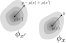
\includegraphics[width=0.35\columnwidth]{mean_displacement_invariance.pdf}
		
		\vspace{1em}
		
		\textbf{Local mean-displacement invariance:}
		$$\phi_x(y) \approx \phi_{x'}(y-\mu(x) + \mu(x'))$$
		
		%\includegraphics[width=0.6\columnwidth]{Hess1_ordered.png}
	\end{center}
\end{frame}


\begin{frame}[t]
	\frametitle{Framework for approximate Hessian entry evaluation}
	\framesubtitle{Illustration of framework by impulse response local-translation invariance}
	\only<1-2>{
		Consider
		\begin{align*}
		\bs{v}^{\top}\bs{K}\bs{u}&=a(u,v):=
		\int_{\Omega}\bs{\nabla}u\cdot\bs{\nabla}v\mathrm{d}x
		\end{align*}
	}
	\begin{align*}
	\onslide<2->{\bs{v}^{\top}\Hmisfit\bs{u}=
		(H_{\text{\tiny misfit}}\,u)(v)&:=
		\int_{\Omega}\int_{\Omega}v(y)\,\Phi(y,x)\,u(x)\mathrm{d}x\,\mathrm{d}y \\}
	\onslide<3->{\Phi(y,x)&\approx \Phi(y+s,x+s) \text{ for small } s \quad\quad (\text{local-translation invariance}) \\}
	\onslide<4->{\underbrace{{\color<6->{teal}{\phi_{x}}}(y)}_{\text{impulse response}}&:=\Phi(y,x)=({\color<7->{magenta}{H_{\text{\tiny misfit}}\,\delta_{x}^{*}}})^{*}\footnotemark\\}
	\onslide<5->{
		\implies \color<5->{purple}{(H_{\text{\tiny misfit}}u)(v)}&\approx 
		\int_{\Omega}v(y)\left(\sum_{i}\int_{\Omega_{i}}{\color<6->{teal}{\phi_{x_{i}^{\prime}}}}(y-x+x_{i}^{\prime})u(x)\mathrm{d}x\right)\mathrm{d}y}	
	\end{align*}
	\only<4->
	{%
		\footnotetext[1]{$\phantom{e}^{*}$ indicates the Riesz representative, that is $\ell^{*}\in L^{2}(\Omega)$ is the Riesz representative of a linear functional $\ell: L^{2}(\Omega)\rightarrow\mathbb{R}$, provided $\ell(w)=(\ell^{*},w)_{L^{2}(\Omega)}$ for each $w\in L^{2}(\Omega)$. $\delta_{x}$ indicates the Dirac distribution with mass concentrated at $x$.}   
	}
	\only<5->
	{%
		\begin{itemize}
			\item[$\star$] \textbf{Key idea:} \only<5->{approximate {\color<5->{purple}{Hessian entries}}} \only<6->{by interpolating a fixed number of {\color{teal}{impulse response functions}},} 
			\only<7->
			{each of which is determined by one {\color{magenta}{Hessian-apply}}.}
		\end{itemize}
	}
	
\end{frame}


\begin{frame}[t]
	\frametitle{Hessian impulse responses (Pine Island Glacier)}
	\center
	\only<1>{
		\begin{center}
			\includegraphics[width=0.7\columnwidth]{reordered_phi/phi0_minimal.png}
		\end{center}
	}
	\only<2>{
		\begin{center}
			\includegraphics[width=0.7\columnwidth]{reordered_phi/phi1_minimal.png}
		\end{center}
	}
	\only<3>{
		\begin{center}
			\includegraphics[width=0.7\columnwidth]{reordered_phi/phi2_minimal.png}
		\end{center}
	}
	\only<4>{
		\begin{center}
			\includegraphics[width=0.7\columnwidth]{reordered_phi/phi3_minimal.png}
		\end{center}
	}
	\only<5>{
		\begin{center}
			\includegraphics[width=0.7\columnwidth]{reordered_phi/phi4_minimal.png}
		\end{center}
	}
	\only<6>{
		\begin{center}
			\includegraphics[width=0.7\columnwidth]{reordered_phi/phi5_minimal.png}
		\end{center}
	}
	\only<7>{
		\begin{center}
			\includegraphics[width=0.7\columnwidth]{reordered_phi/phi6_minimal.png}
		\end{center}
	}
	\only<8>{
		\begin{center}
			\includegraphics[width=0.7\columnwidth]{reordered_phi/phi7_minimal.png}
		\end{center}
	}
	\only<9>{
		\begin{center}
			\includegraphics[width=0.7\columnwidth]{reordered_phi/phi8_minimal.png}
		\end{center}
	}
	\only<10>{
		\begin{center}
			\includegraphics[width=0.7\columnwidth]{reordered_phi/phi9_minimal.png}
		\end{center}
	}
	\only<11>{
		\begin{center}
			\includegraphics[width=0.7\columnwidth]{reordered_phi/phi10_minimal.png}
		\end{center}
	}
	\only<12>{
		\begin{center}
			\includegraphics[width=0.7\columnwidth]{reordered_phi/phi11_minimal.png}
		\end{center}
	}
	\only<13>{
		\begin{center}
			\includegraphics[width=0.7\columnwidth]{reordered_phi/phi12_minimal.png}
		\end{center}
	}
	\only<14>{
		\begin{center}
			\includegraphics[width=0.7\columnwidth]{reordered_phi/phi13_minimal.png}
		\end{center}
	}
	\only<15>{
		\begin{center}
			\includegraphics[width=0.7\columnwidth]{reordered_phi/phi14_minimal.png}
		\end{center}
	}
	\only<16>{
		\begin{center}
			\includegraphics[width=0.7\columnwidth]{reordered_phi/phi15_minimal.png}
		\end{center}
	}
	\only<17>{
		\begin{center}
			\includegraphics[width=0.7\columnwidth]{reordered_phi/phi16_minimal.png}
		\end{center}
	}
	\only<18>{
		\begin{center}
			\includegraphics[width=0.7\columnwidth]{reordered_phi/phi17_minimal.png}
		\end{center}
	}
	\only<19>{
		\begin{center}
			\includegraphics[width=0.7\columnwidth]{reordered_phi/phi18_minimal.png}
		\end{center}
	}
	\only<20>{
		\begin{center}
			\includegraphics[width=0.7\columnwidth]{reordered_phi/phi19_minimal.png}
		\end{center}
	}
	\only<21>{
		\begin{center}
			\includegraphics[width=0.7\columnwidth]{reordered_phi/phi20_minimal.png}
		\end{center}
	}
	\only<22>{
		\begin{center}
			\includegraphics[width=0.7\columnwidth]{reordered_phi/phi21_minimal.png}
		\end{center}
	}
	\only<23>{
		\begin{center}
			\includegraphics[width=0.7\columnwidth]{reordered_phi/phi22_minimal.png}
		\end{center}
	}
	\only<24>{
		\begin{center}
			\includegraphics[width=0.7\columnwidth]{reordered_phi/phi23_minimal.png}
		\end{center}
	}
	\only<25>{
		\begin{center}
			\includegraphics[width=0.7\columnwidth]{reordered_phi/phi24_minimal.png}
		\end{center}
	}
	\only<26>{
		\begin{center}
			\includegraphics[width=0.7\columnwidth]{reordered_phi/phi25_minimal.png}
		\end{center}
	}
	\only<27>{
		\begin{center}
			\includegraphics[width=0.7\columnwidth]{reordered_phi/phi26_minimal.png}
		\end{center}
	}
	\only<28>{
		\begin{center}
			\includegraphics[width=0.7\columnwidth]{reordered_phi/phi27_minimal.png}
		\end{center}
	}
	\only<29>{
		\begin{center}
			\includegraphics[width=0.7\columnwidth]{reordered_phi/phi28_minimal.png}
		\end{center}
	}
	\only<30>{
		\begin{center}
			\includegraphics[width=0.7\columnwidth]{reordered_phi/phi29_minimal.png}
		\end{center}
	}
	\only<31>{
		\begin{center}
			\includegraphics[width=0.7\columnwidth]{reordered_phi/phi30_minimal.png}
		\end{center}
	}
	\only<32>{
		\begin{center}
			\includegraphics[width=0.7\columnwidth]{reordered_phi/phi31_minimal.png}
		\end{center}
	}
	\only<33>{
		\begin{center}
			\includegraphics[width=0.7\columnwidth]{reordered_phi/phi32_minimal.png}
		\end{center}
	}
	\only<34>{
		\begin{center}
			\includegraphics[width=0.7\columnwidth]{reordered_phi/phi33_minimal.png}
		\end{center}
	}
	\only<35>{
		\begin{center}
			\includegraphics[width=0.7\columnwidth]{reordered_phi/phi34_minimal.png}
		\end{center}
	}
	\only<36>{
		\begin{center}
			\includegraphics[width=0.7\columnwidth]{reordered_phi/phi35_minimal.png}
		\end{center}
	}
	\only<37>{
		\begin{center}
			\includegraphics[width=0.7\columnwidth]{reordered_phi/phi36_minimal.png}
		\end{center}
	}
	\only<38>{
		\begin{center}
			\includegraphics[width=0.7\columnwidth]{reordered_phi/phi37_minimal.png}
		\end{center}
	}
	\only<39>{
		\begin{center}
			\includegraphics[width=0.7\columnwidth]{reordered_phi/phi38_minimal.png}
		\end{center}
	}
	\only<40>{
		\begin{center}
			\includegraphics[width=0.7\columnwidth]{reordered_phi/phi39_minimal.png}
		\end{center}
	}
	\only<41>{
		\begin{center}
			\includegraphics[width=0.7\columnwidth]{reordered_phi/phi40_minimal.png}
		\end{center}
	}
	\only<42>{
		\begin{center}
			\includegraphics[width=0.70\columnwidth]{reordered_phi/phi41_minimal.png}
		\end{center}
	}
	\only<43>{
		\begin{center}
			\includegraphics[width=0.7\columnwidth]{reordered_phi/phi42_minimal.png}
		\end{center}
	}
	\only<44>{
		\begin{center}
			\includegraphics[width=0.7\columnwidth]{reordered_phi/phi43_minimal.png}
		\end{center}
	}
	\only<45>{
		\begin{center}
			\includegraphics[width=0.7\columnwidth]{reordered_phi/phi44_minimal.png}
		\end{center}
	}
	\only<46>{
		\begin{center}
			\includegraphics[width=0.7\columnwidth]{reordered_phi/phi45_minimal.png}
		\end{center}
	}
	\only<47>{
		\begin{center}
			\includegraphics[width=0.7\columnwidth]{reordered_phi/phi46_minimal.png}
		\end{center}
	}
	\only<48>{
		\begin{center}
			\includegraphics[width=0.7\columnwidth]{reordered_phi/phi47_minimal.png}
		\end{center}
	}
	\only<49>{
		\begin{center}
			\includegraphics[width=0.7\columnwidth]{reordered_phi/phi48_minimal.png}
		\end{center}
	}
	\only<50>{
		\begin{center}
			\includegraphics[width=0.7\columnwidth]{reordered_phi/phi49_minimal.png}
		\end{center}
	}
	\only<51>{
		\begin{center}
			\includegraphics[width=0.7\columnwidth]{reordered_phi/phi50_minimal.png}
		\end{center}
	}
	\only<52>{
		\begin{center}
			\includegraphics[width=0.7\columnwidth]{reordered_phi/phi51_minimal.png}
		\end{center}
	}
	\only<53>{
		\begin{center}
			\includegraphics[width=0.7\columnwidth]{reordered_phi/phi52_minimal.png}
		\end{center}
	}
	\only<54>{
		\begin{center}
			\includegraphics[width=0.7\columnwidth]{reordered_phi/phi53_minimal.png}
		\end{center}
	}
	\only<55>{
		\begin{center}
			\includegraphics[width=0.7\columnwidth]{reordered_phi/phi54_minimal.png}
		\end{center}
	}
	\only<56>{
		\begin{center}
			\includegraphics[width=0.7\columnwidth]{reordered_phi/phi55_minimal.png}
		\end{center}
	}
	\only<57>{
		\begin{center}
			\includegraphics[width=0.7\columnwidth]{reordered_phi/phi56_minimal.png}
		\end{center}
	}
	\only<58>{
		\begin{center}
			\includegraphics[width=0.7\columnwidth]{reordered_phi/phi57_minimal.png}
		\end{center}
	}
	\only<59>{
		\begin{center}
			\includegraphics[width=0.7\columnwidth]{reordered_phi/phi58_minimal.png}
		\end{center}
	}
	\only<60>{
		\begin{center}
			\includegraphics[width=0.7\columnwidth]{reordered_phi/phi59_minimal.png}
		\end{center}
	}
	\only<61>{
		\begin{center}
			\includegraphics[width=0.7\columnwidth]{reordered_phi/phi60_minimal.png}
		\end{center}
	}
	\only<62>{
		\begin{center}
			\includegraphics[width=0.7\columnwidth]{reordered_phi/phi61_minimal.png}
		\end{center}
	}
	\only<63>{
		\begin{center}
			\includegraphics[width=0.7\columnwidth]{reordered_phi/phi62_minimal.png}
		\end{center}
	}
	\only<64>{
		\begin{center}
			\includegraphics[width=0.7\columnwidth]{reordered_phi/phi63_minimal.png}
		\end{center}
	}
	\only<65>{
		\begin{center}
			\includegraphics[width=0.7\columnwidth]{reordered_phi/phi64_minimal.png}
		\end{center}
	}
	\only<66>{
		\begin{center}
			\includegraphics[width=0.7\columnwidth]{reordered_phi/phi65_minimal.png}
		\end{center}
	}
	\only<67>{
		\begin{center}
			\includegraphics[width=0.7\columnwidth]{reordered_phi/phi66_minimal.png}
		\end{center}
	}
	\only<68>{
		\begin{center}
			\includegraphics[width=0.7\columnwidth]{reordered_phi/phi67_minimal.png}
		\end{center}
	}
	\only<69>{
		\begin{center}
			\includegraphics[width=0.7\columnwidth]{reordered_phi/phi68_minimal.png}
		\end{center}
	}
	
\end{frame}



\begin{frame}
	\frametitle{Impulse responses are ``columns'' of the integral kernel}
	\begin{center}
		
		\includegraphics[width=0.5\columnwidth]{kernel_impulse_illustration2.pdf}
		
	\end{center}
\end{frame}



%---------------------------------------------------------------------------------%
\begin{frame}[t]
	\frametitle{Hessian approximation method: big idea}
	\begin{itemize}
		\item {\bf Step 1:} Compute ``batches'' of impulse responses by applying Hessian to Dirac combs
		\item {\bf Step 2:} Interpolate known impulse responses to approximate unknown Hessian entries $\mathbf{H}_{ij}$
		\item {\bf Step 3:} Convert to $\mathcal{H}$-matrix to do linear algebra (with low computational complexity)
	\end{itemize}
    \begin{figure} 
	\includegraphics[width=0.375\columnwidth]{impulse_batch1.png} \hfil  
	\includegraphics[width=0.375\columnwidth]{impulse_batch2.png}
	\end{figure} 
	*Impulse response batches from Ice Mountain
\end{frame}
%---------------------------------------------------------------------------------%

%---------------------------------------------------------------------------------%
\begin{frame}[t]
	\frametitle{How to choose impulse response points?}
	
	\begin{columns}
		\begin{column}{0.5\columnwidth}
			One Hessian-vector product can yield many impulse responses (with small region of support)
		\begin{center}
			\includegraphics[width=0.75\columnwidth]{impulse_batch2.png} 
		\end{center}
	    \end{column}
    \begin{column}{0.49\columnwidth}
    	\only<2>
    	{ 
		\begin{itemize}
			\item \textbf{Goal:} determine as many points as possible, such that the associated impulse response supports do not overlap
			\item \textbf{Dilemma:} how can we know the impulse response supports before we compute them?
		\end{itemize}
	    }
	\end{column} 
	\end{columns}

\end{frame}
%---------------------------------------------------------------------------------%
\begin{frame}
	\frametitle{Matrix analogy: getting all row sums}
	
	\textbf{Matrix:} let $\mathbf{A} \in \mathbb{R}^{N \times N}$. Then
	
	$$\mathbf{A}^{\top} \begin{bmatrix}
	1 \\ 1 \\ \vdots \\ 1
	\end{bmatrix} = \begin{bmatrix}
	\text{sum of }\mathbf{A} \text{ col }1 \\
	\text{sum of }\mathbf{A} \text{ col }2 \\
	\vdots \\
	\text{sum of }\mathbf{A} \text{ col }N
	\end{bmatrix}$$
	
	Sum of each row obtained by transpose apply to vector of ones
	
	\vspace{3em}
	
	\textbf{Operator:} let $C(x)=1$ be the constant function. Then 
	
	$$(H_{\text{\tiny misfit}}^{\dagger} C)^*(y) = \int_\Omega \left(H_{\text{\tiny misfit}} \delta_y\right)(x) \,\mathrm{d}x=\int_{\Omega}\phi_{y}(x)\,\mathrm{d}x$$
	
	
	Volume of each impulse response obtained by adjoint Hessian operator apply to constant function
\end{frame}
%---------------------------------------------------------------------------------%
\begin{frame}
	\frametitle{Mean and standard deviations of impulse responses}
	\begin{itemize}
		\setlength\itemsep{2em}
		\item Let $V(x)$, $\mu(x)$, and $\Sigma(x)$ be the ``volume'', ``mean'', and ``variance'' of $\phi_x$
		\item Let $C$, $L^i$, and $Q^{ij}$ be the following functions:
		\begin{equation*}
		C(x) := 1, \qquad
		L^i(x) := x^i, \qquad
		Q^{ij}(x) = x^i x^j
		\end{equation*}
		\item Then
		\begin{align*}
		V =& \left(H_{\text{\tiny misfit}}^{\dagger} C\right)^* \\
		\mu^i =& \left(H_{\text{\tiny misfit}}^{\dagger} L^i\right)^* / V \\
		\Sigma^{ij} =& \left(H_{\text{\tiny misfit}}^{\dagger} Q^{ij}\right)^* / V - \mu^i\cdot \mu^j
		\end{align*}
		\item Estimates of impulse response supports obtained from 
		first few moments (adjoint Hessian apply to constant, linear, and quadratic functions)
	\end{itemize}
	
\end{frame}
%---------------------------------------------------------------------------------%
\begin{frame}
	\frametitle{Impulse response support ellipsoids}
	\begin{itemize}
		\item $\phi_x$ is \textbf{approximately supported} in the ellipsoid
		$$E = \{y: (y - \mu(x))^T\Sigma(x)^{-1}(y - \mu(x)) \le \tau^2\}$$
		
		\item Picking impulse response points becomes an \textbf{ellipsoid packing problem}
		
		\item Pack ellipsoids using \textbf{greedy algorithm}
	\end{itemize}
	\begin{center}
		\includegraphics[width=0.375\columnwidth]{impulse_batch2.png} 
	\end{center}
\end{frame}


\begin{frame}
	\frametitle{Computational cost}
	\begin{itemize}
		\setlength\itemsep{2em}
		\item \textbf{Hessian-vector products:} 
		$$1+\text{dim}(\Omega)(\text{dim}(\Omega)+3)/2 + n_\text{batches}$$
		E.g., $11$ Hessian-vector products for $5$ batches of impulse responses and $\text{dim}(\Omega)=2$
		\item \textbf{Ellipsoid intersection tests:}
		$$O(Nm)$$
		where $m$ is total number of impulse responses in all batches
		\item \textbf{Elementary operations} to build and use the $\mathcal{H}$-matrix:
		$$O(N \log N)$$ 
	\end{itemize}
\end{frame}


%---------------------------------------------------------------------------------%

%\begin{frame}
%	\frametitle{Boundary considerations (1)}
%	\begin{center}
%		\includegraphics[width=0.8\textwidth]{interpolation_rbf_boundary.pdf}
%	\end{center}
%	\begin{itemize}
%		\item If $p_i + y - x$ is outside the domain, don't use $i$th impulse response for $H(y,x)$
%	\end{itemize}
%\end{frame}
%---------------------------------------------------------------------------------%

%\begin{frame}
%	\frametitle{Boundary considerations (2)}
%	\begin{center}
%		\includegraphics[width=0.8\textwidth]{interpolation_rbf_adjoint.pdf}
%	\end{center}
%	\begin{itemize}
%		\item Take advantage of symmetry
%	\end{itemize}
%\end{frame}
%---------------------------------------------------------------------------------%

%---------------------------------------------------------------------------------%
%\begin{frame}
%	\frametitle{How to choose impulse response points?}
%	One hessian matrix-vector product $\rightarrow$ many impulse responses
%	\begin{center}
%		\includegraphics[width=0.5\columnwidth]{IRB1.png} 
%	\end{center}
%	\begin{itemize}
%		\item \textbf{Goal:} choose as many points as possible, such that the impulse response supports don't overlap
%		\item \textbf{Dilemma:} How can we know the impulse response supports before we compute them?
%	\end{itemize}
%\end{frame}
%---------------------------------------------------------------------------------%

%---------------------------------------------------------------------------------%

%---------------------------------------------------------------------------------%

%---------------------------------------------------------------------------------%
%\begin{frame}
%	\frametitle{Ice Mountain: Setup}
%	\begin{figure}
%		\begin{center} 
%			\begin{subfigure}{0.99\textwidth}
%				\begin{center} 
%					\includegraphics[scale=0.2]{meshHeight_view2_edges.png} \hfil
%				\end{center}
%				\caption{Ice sheet model geometry}
%				\label{fig:ice_mountain_mesh}
%			\end{subfigure} \\
%			\begin{subfigure}{0.49\textwidth}
%				\includegraphics[scale=0.2]{mtrue_withColorBar.png}
%				\caption{$\beta_\text{true}$}
%				\label{fig:true_beta}
%			\end{subfigure}
%			\begin{subfigure}{0.49\textwidth}
%				\includegraphics[scale=0.2]{trueVelocity2_glyphs.png}
%				\caption{$v_\text{true}$}
%				\label{fig:stokes_velocity}
%			\end{subfigure}
%		\end{center}
%	\end{figure} 
%\end{frame}
\begin{frame}
	\frametitle{Example: ``Ice mountain'' inverse problem}
	
	\begin{figure}
		\centering\includegraphics[scale=0.22]{figures/meshHeight_view2_edges.png}\\
		\includegraphics[scale=0.18]{figures/mtrue_withColorBar.png}
		\includegraphics[scale=0.18]{figures/trueVelocity2_glyphs.png}
	\end{figure}
	\begin{center}
		The ice sheet geometry and discretization (top), the ``true''
		parameter (bottom left) and the corresponding velocity field
		(bottom right).
	\end{center}
\end{frame}
%---------------------------------------------------------------------
\begin{frame}
	\frametitle{Example: ``Ice mountain'' inverse problem}
	\framesubtitle{Impulse responses}
	
	\begin{figure}
		\includegraphics[width=0.32\columnwidth]{figures/impulse_batch1.png}
		\includegraphics[width=0.32\columnwidth]{figures/impulse_batch2.png}
		\includegraphics[width=0.32\columnwidth]{figures/impulse_batch3.png}
	\end{figure}
	
	%\footnotesize
	\begin{itemize}
		\item Black stars are point source locations.
		\item Shading shows the magnitude of the normalized impulse
		responses.
		\item Dashed gray ellipses are estimated impulse
		response support ellipsoids based on the moment method.
	\end{itemize}
	
\end{frame}
%---------------------------------------------------------------------
\begin{frame}
	\frametitle{Example: ``Ice mountain'' inverse problem}
	
	\begin{figure}
		%[width=0.8\columnwidth]
		\centering\includegraphics[scale=0.6]{extraplots/reconstructions-ice.png}
		%\centering\includegraphics[scale=0.18]{figures/mstar_0.25noise_cropped.png}
		%\includegraphics[scale=0.18]{figures/mstar_0.05noise_cropped.png}
		%\includegraphics[scale=0.18]{figures/mstar_0.01noise_cropped.png}
	\end{figure}
	\begin{center}
		The log basal sliding parameter computed from the PDE-constrained
		optimization problem with noise levels: $25\%$ (left), $5.0\%$
		(middle), and $1.0\%$ (right).
	\end{center}
\end{frame}
%---------------------------------------------------------------------
\begin{frame}
	\frametitle{Example: ``Ice mountain'' inverse problem}
	\framesubtitle{Convergence history for solving the Stokes inverse problem using inexact Newton PCG}
	
	\only<1>{
		\begin{table}
			{\small
				\begin{center}
					\begingroup
					\setlength{\tabcolsep}{3pt}
					\renewcommand{\arraystretch}{1.1}
					\begin{tabular}{c| c c c | c c c | c c c}
						&  \multicolumn{3}{|c|}{PSF (5)} & \multicolumn{3}{|c|}{REG} & \multicolumn{3}{|c}{NONE} \\
						\hline
						Iter & 
						\#CG & \#Stokes & $\|\mathbf{g}\|$ & 
						\#CG & \#Stokes & $\|\mathbf{g}\|$ & 
						\#CG & \#Stokes & $\|\mathbf{g}\|$ \\
						0 &
						1 & 4 & 1.9e+7 &
						3 & 8 & 1.9e+7 &
						1 & 4 & 1.9e+7 \\
						1 &
						2 & 6  & 6.1e+6 &
						8 & 18 & 8.4e+6 &
						2 & 6  & 6.1e+6 \\
						2 &
						4 & 10 & 2.6e+6 &
						16 & 34 & 4.1e+6 &
						4 & 10 & 2.6e+6 \\
						3 &
						2 & 6+22 & 6.9e+5 &
						34 & 70 & 1.8e+6 &
						14 & 30 & 6.9e+5 \\
						4 &
						3 & 8 & 4.4e+4 &
						52 & 106 & 5.6e+5 &
						29 & 60 & 1.3e+5 \\
						5 &
						5 & 12 & 2.2e+3 &
						79 & 160 & 9.4e+4 &
						38 & 78 & 1.0e+4 \\
						6 &
						0 & 2 & 1.1e+1 &
						102 & 206 & 6.5e+3 &
						58 & 118 & 1.8e+2 \\
						7 &
						--- & --- & --- &
						151 & 304 & 1.2e+2 &
						0 & 2 & 5.5e-1 \\
						8 & 
						--- & --- & --- &
						0 & 2 & 2.9e-1 &
						--- & --- & --- \\
						\hline
						Total & 
						17 & 70 & --- &
						445 & 908 & --- &
						146 & 308 & --- \\
					\end{tabular}
					\endgroup
				\end{center}
			}
		\end{table}
	}
	
	\only<2>{
		\begin{table}
			{\small
				\begin{center}
					\begingroup
					\setlength{\tabcolsep}{3pt}
					\renewcommand{\arraystretch}{1.1}
					\begin{tabular}{c| c c c | c c c | c c c}
						&  \multicolumn{3}{|c|}{PSF (5)} & \multicolumn{3}{|c|}{REG} & \multicolumn{3}{|c}{NONE} \\
						\hline
						Iter & 
						\#CG & \#Stokes & $\|\mathbf{g}\|$ & 
						\#CG & \#Stokes & $\|\mathbf{g}\|$ & 
						\#CG & \#Stokes & $\|\mathbf{g}\|$ \\
						0 &
						1 & 4 & 1.9e+7 &
						3 & 8 & 1.9e+7 &
						1 & 4 & 1.9e+7 \\
						1 &
						2 & 6  & 6.1e+6 &
						8 & 18 & 8.4e+6 &
						2 & 6  & 6.1e+6 \\
						2 &
						4 & 10 & 2.6e+6 &
						16 & 34 & 4.1e+6 &
						4 & 10 & 2.6e+6 \\
						3 &
						2 & 6+22 & 6.9e+5 &
						34 & 70 & 1.8e+6 &
						14 & 30 & 6.9e+5 \\
						4 &
						3 & 8 & 4.4e+4 &
						52 & 106 & 5.6e+5 &
						29 & 60 & 1.3e+5 \\
						5 &
						5 & 12 & 2.2e+3 &
						79 & 160 & 9.4e+4 &
						38 & 78 & 1.0e+4 \\
						6 &
						0 & 2 & 1.1e+1 &
						102 & 206 & 6.5e+3 &
						58 & 118 & 1.8e+2 \\
						7 &
						--- & --- & --- &
						151 & 304 & 1.2e+2 &
						0 & 2 & 5.5e-1 \\
						8 & 
						--- & --- & --- &
						0 & 2 & 2.9e-1 &
						--- & --- & --- \\
						\hline
						Total & 
						17 & {\bf \alert{70}} & --- &
						445 & {\bf \alert{908}} & --- &
						146 & {\bf \alert{308}} & --- \\
					\end{tabular}
					\endgroup
				\end{center}
			}
		\end{table}  
	}
	
	\footnotesize
	\begin{itemize}
		\item \#CG:  the number of PCG iterations used to solve the Newton system.
		\item \#Stokes: the total number of Stokes PDE solves performed in each Newton iteration.
		\item $\|\mathbf{g}\|$: the Euclidean norm of the gradient.
	\end{itemize}
\end{frame}
%---------------------------------------------------------------------
\begin{frame}
	\frametitle{Example: ``Ice mountain'' inverse problem}
	\framesubtitle{Convergence history and eigenvalue clustering}
	
	\begin{figure}
		\begin{center}
			\includegraphics[width=0.75\columnwidth]{extraplots/bbb}
		\end{center}
	\end{figure}
	%\begin{center}
		Left: convergence history for solving $\mathbf{H} \mathbf{x} = \mathbf{b}$
		using PCG, where $\mathbf{b}$ has i.i.d. random entries and $\mathbf{H}$ is evaluated at the
		solution of the inverse problem. \\ Right: generalized eigenvalues
		for generalized eigenvalue problem $\mathbf{H} \mathbf{u}_{k}=\lambda_{k}
		\mathbf{\preconditioner} \mathbf{u}_{k}$.
	%\end{center}
\end{frame}
%---------------------------------------------------------------------
\begin{frame}
	\frametitle{Example: ``Ice mountain'' inverse problem}
	\framesubtitle{Condition number of preconditioned Hessian}
	
	\begin{table}
		\begin{center}
			\begingroup
			\setlength{\tabcolsep}{4pt}
			\renewcommand{\arraystretch}{1.25}
			\begin{tabular}{c| c c c c c}
				noise    & \multicolumn{5}{c}{COND$(\mathbf{\preconditioner}^{-1} \mathbf{H})$ } \\ \cline{2-6}
				level    & REG     &	NONE  & PSF $(1)$ & PSF $(5)$ & PSF $(25)$ \\ \hline 
				$25\%$   & 1.01e+3 & 2.96e+3  & 1.34e+0   & 1.30e+0   & 1.18e+0    \\ 
				$11\%$   & 7.40e+3 & 1.05e+3  & 2.27e+0   & 1.55e+0   & 1.31e+0    \\   
				$5.0\%$  & 3.29e+4 & 4.96e+2  & 5.61e+0   & 3.06e+0   & 1.92e+0    \\ 
				$2.2\%$  & 1.66e+5 & 8.89e+2  & 1.58e+1   & 8.07e+0   & 4.03e+0    \\  
				$1.0\%$  & 5.36e+5 & 1.61e+3  & 7.17e+1   & 1.93e+1   & 9.19e+0    \\   
			\end{tabular}
			\endgroup
		\end{center}
	\end{table}
	
	%\begin{center}
		Condition number for $\mathbf{\preconditioner}^{-1} \mathbf{H}$ for
		the PSF-based preconditioners with 1, 5, and 25 batches (PSF (1),
		PSF (5), and PSF(25), respectively), no preconditioner (NONE) and
		regularization (REG).
	%\end{center}  
\end{frame}




\begin{frame}
	\frametitle{Summary}
	
	\begin{itemize}
		\setlength\itemsep{1.5em}
		\item Hessian approximations or preconditioners are essential for solution of Bayesian inverse problems governed by
		partial differential equations.
		\vspace{0.05in}
		\item Low-rank approximations of the Hessian become
		prohibitive as the data becomes more informative, as is the case
		for continental-scale ice sheet inverse problems.
		\vspace{0.05in}
		\item Local point spread function interpolation combined with hierarchical matrix representations promise a more efficient
		Hessian approximation.
	\end{itemize}
	\vspace{2em}
	{\small Alger, N., Hartland, T., Petra, N., Ghattas, O. (2024). Point spread function approximation of high rank Hessians with locally supported non-negative integral kernels. To appear in SISC.}
\end{frame}



\end{document}
